\section{Experiment}
\label{sec:exp}

We compare the results of news and tweets by \stlda and conventional LDA models respectively, and evaluate the quality of topic assignments. Then based on the results by \stlda, we compare the topic dynamics between tweets in and out \stlouis area and examine the geographic difference in topics regarding to Ferguson Unrest. Daily proportion of diverse topics for news and tweets are examined to understand the coverage difference and interaction between news and tweets.

\subsection{Dataset}

We collected 13,238,863 tweets from August 10, 2014 to August 27, 2014 mentioning Ferguson using the Twitter Streaming API. Among them 92,184 are geo-tagged, which takes about 0.70\% of all. We use geo-tagged tweets instead of all tweets because an empirical study~\cite{he2015uncovering} shows that there is geographic difference in tweet topics for a certain event. Meanwhile there is not much difference in the reaction time, volume, and topics between geo-tagged tweets and non geo-tagged tweets. So we use geo-tagged tweets to analyze topics in different areas, in representative of general public opinions. To assist geographic analysis, we use 2014 TIGER/Lines Shapefile to identify the locations of tweets according to tweets' coordinates.\footnote{\url{https://www.census.gov/geo/maps-data/data/tiger-line.html}}

News is crawled by the links published by news account on Twitter. We randomly selected 108 media accounts from Twitter, for example ``Washington Post", ``NBC News" and ``ABC7News", collected all the tweets they published during the Ferguson event, and extracted news reports from the links they published. In total, there are 1,338 news covering from August 11 to 27.

Same standard preprocessing procedure is applied to news and Twitter corpora, such as tokenization, POS tagging, lemmatization, bigrams detection, stop words, low frequency words and too high frequency words removal. However, we use different tools for the two corpora: OpenNLP package~\cite{baldridge2005opennlp} for news corpus and Tweet NLP package~\cite{owoputi2013improved} for Twitter corpus. After preprocessing and removing empty documents, there are 1,275 news documents and 81,553 Twitter documents, as well as a vocabulary with 1,132 words.

\subsection{Discovery of Topic Dynamics}

\stlda is able to train long (news) and short documents (tweets) simultaneously, by assigning multiple topics to long documents and one topic to short documents. The output results of \stlda model can be used for further discovery of topic dynamics of tweets and news. We define topic dynamics as temporal change of topics using daily sliding window. Assuming that every news document has the same impact and contributes equally to the total media environment, the topic proportion of day $t$ is the average of topic probabilities of all news documents on that day as

\begin{equation}
\bar{\theta}_{t,k}^{\mathrm{news}}=\frac{\sum_{d=1}^{D_t^{\mathrm{news}}} \theta_{d,k}}{D_t^{\mathrm{news}}},
\end{equation}
where $D_t^{\mathrm{news}}$ denotes the number of news documents on day $t$; $\theta_{d,k}$ is topic $k$'s proportion in document $d$.

Differently, each tweet $d$ has only one topic $z_d$ given by \stlda. Under the same assumption that each tweet contributes equally to the voice of public, the aggregation of daily tweet topic proportion is calculated as

\begin{equation}
\bar{\theta}_{t,k}^{\mathrm{tweets}} = \frac{\sum_{d=1}^{D_t^{\mathrm{tweets}}} \mathbbm{1}(z_d=k)}{D_t^{\mathrm{tweets}}},
\end{equation}
where $D_t^{\mathrm{tweets}}$ denotes the number of tweet documents on day $t$ and $\mathbbm{1}(\cdot)$ is an indicator function.

Given $\bm{\bar{\theta}_t^{\mathrm{news}}}$ and $\bm{\bar{\theta}_t^{\mathrm{tweets}}}$ where $t$ varies from August 11 to 27, we can identify topic dynamics by the changing of daily topic proportions.


\subsection{Topic Quality Evaluation}

In this section, we compare the performance by evaluating the topic quality given by LDA and \stlda both intrinsically and extrinsically. The hyperparameters $\alpha$ and $\beta$ are both set to 0.1 and the number of topics is set to 10.

As topics given by two models are in different orders, we match the topics based on KL divergence before comparing them. The matching procedure starts by obtaining a KL divergence table $T$. Each cell $T_{k_1,k_2}$ stores the KL divergence of topic $k_1$ given by LDA and topic $k_2$ given by \stlda as

\begin{eqnarray}
T_{k_1,k_2}&=&\mathrm{KL}(\bm{\phi_{k_1}^\mathrm{LDA}}||\bm{\phi_{k_2}^\mathrm{\stlda}})\\
&=&\sum_{v=1}^{V} \phi_{k_1,v}^{\mathrm{LDA}} \log_2 \frac{\phi_{k_1,v}^{\mathrm{LDA}}}{\phi_{k_2,v}^{\mathrm{\stlda}}}.
\end{eqnarray}

Then we run a depth-first search algorithm on the KL divergence table to find the best match which has the smallest the overall KL divergence.

\subsubsection{Comparison of Topics}

\begin{table*}[htpb]
\centering
\begin{threeparttable}
\begin{tabular}{|c|c|l|}
\hline
\bf \tabincell{c}{Model\\(Corpus)} & \bf Topic & \multicolumn{1}{c|}{\bf Top Words}\\ \hline
\multirow{5}*{\tabincell{c}{LDA\\(NT)\tnote{1}}} & Obama Talk & happen, i'm, make, thing, talk, situation, what's, what's\_happen, bad, you're\\ \cline{2-3}
 & Protest & tear\_gas, protester, arrest, fire, medium, rt, protestor, street, crowd\\ \cline{2-3}
 & Racist & black, white, loot, protect, community, racist, stop, race, citizen, riot\\ \cline{2-3}
 & Curfew & missouri, state, obama, national\_guard, call, curfew, mo, press, governor\\ \cline{2-3}
 & Pray & peace, pray, justice, stand, love, tonight, hope, stay, family, safe\\ \hline
\multirow{5}*{\tabincell{c}{\stlda\\(NT)}} & Obama Talk & obama, president, law\_enforcement, house, holder, make, story, post, include\\ \cline{2-3}
 & Protest & tear\_gas, arrest, protester, fire, rt, reporter, medium, shoot, crowd\\ \cline{2-3}
 & Racist & black, white, make, race, america, obama, stop, happen, situation, riot\\ \cline{2-3}
 & Curfew & missouri, curfew, state, national\_guard, governor, nixon, call, gov, order\\ \cline{2-3}
 & Pray & peace, pray, stand, justice, night, love, tonight, today, family\\ \hline
\multirow{5}{*}{\tabincell{c}{LDA\\(N)\tnote{2}}} & Obama Talk & obama, president, house, make, white, news, national, deal, run, defense\\ \cline{2-3}
 & Protest & st\_louis, nixon, protester, shooting, county, justice, aug., investigation, state, thursday\\ \cline{2-3}
 & Racist & black, make, white, cop, time, don't, year, good, man, thing\\ \cline{2-3}
 & Curfew & protester, johnson, tear\_gas, crowd, curfew, night, fire, street, missouri, shoot\\ \cline{2-3}
 & Pray & (No matching topic)\\ \hline
\end{tabular}
\begin{tablenotes}
\footnotesize
\item[1] NT: news and tweets.
\item[2] N: news only.
\end{tablenotes}
\caption{Topic Examples}\label{tab:topic}
\end{threeparttable}
\end{table*}

To evaluate topic quality, we select the top words under each topic. Because news and tweets are trained together with imbalanced number of documents, it is possible that both models may be biased for one type of documents, thus topics may come from only news or tweets. To ensure that both LDA and \stlda have balanced topics that come from tweets and news, we train another model merely on news and set the results as a baseline for comparison.

Table~\ref{tab:topic} shows four common topics for all three models and one topic that only exists in results trained on news and tweets together. Four common topics indicate that news topics are kept when mixture of documents are trained together. But for the one topic \emph{Pray}, there is no matching topic in results of LDA on news, which tends to be the topic that only exists in tweets. It is also worth noting that top words in the four common topics are different. Top words in LDA on news tend to be more complicated and in written language style, such as \emph{justice} and \emph{investigation}. But top words in the topics by mixture texts are a little different. There are oral phrases, such as \emph{i'm} and \emph{you're}, and words which are highly probable to come from tweets such as \emph{rt} and \emph{gov}. These Twitter words indicate that such topics are also covered by tweets. So we can conclude that \stlda can extract topics from both tweets and next, not biased to one type of texts, and it discovers topics that are common in both news and tweets. However, according to analysis of coverage of topics and top words, there is not much difference between LDA and \stlda. It just verifies that there is not extreme bias for either type of texts when trained together. In Section~\ref{subsubsec:intrinsic}, we evaluate the quality of tweets' topics as an intrinsic evaluation. Extrinsic evaluation is applied in Section~\ref{subsubsec:extrinsic}, by using two models in discovery of topic dynamics.

\subsubsection{Topic Quality for Tweets}
\label{subsubsec:intrinsic}

To examine the quality of topic assignment, the most intuitive way is to pick a document and see whether the topic distribution is reasonable to represent the content. Because news is long and contains mixture of latent topics, it is hard to decide whether the topic distribution is appropriate. On the other hand, a tweet is usually constituted by one or two sentences, so it is intuitive to evaluate whether the topic assignment is appropriate.

We list five tweets in Table~\ref{tab:tweets} and their topic distributions by LDA and topic assignments by \stlda are given in Table~\ref{tab:tweet_topic}. Topics in LDA and \stlda are matched and numbered from 0 to 9. Topic names are manually summarized according to top frequency words in the topic.

\begin{table*}[htpb]
\centering
\begin{tabular}{|c|p{14cm}|}
\hline
\bf No. & \multicolumn{1}{c|}{\bf Content}\\ \hline
1 & ``@bkesling: ``Hands up, don't shoot" after tear gas fired in \#Ferguson http://t.co/9zQIh31wQg" modern day America...  \#PrayForFerguson\\ \hline
2 & 80\% black folks think \#Ferguson raises ``important issues about race that need to be discussed," only 37\% of white folks do. Very sad.\\ \hline
3 & You guys can't blame that cop in \#Ferguson. Shooting your gun 6 times is literally the answer to every question in their training manual.\\ \hline
4 & \#fergusongate media get it straight. U act like those who don't live in ferguson can't protest. This is for all blacks everywhere.\\ \hline
5 & But thank God for social media though. Imagine if we're dependent on the news to tell the ``truth" about what's really happening in \#Ferguson\\ \hline
\end{tabular}
\caption{Tweet Examples}\label{tab:tweets}
\end{table*}

\begin{table*}[htpb]
\centering
\begin{tabular}{|c|c|c|c|c|c|c|c|}
\hline
\multicolumn{3}{|c|}{\bf Tweets} & 1 & 2 & 3 & 4 & 5\\ \hline
\multirow{10}{*}{\tabincell{c}{\bf LDA Topic\\ \bf Distribution}} & 0 & Obama Talk & 0.017 & \bf 0.373 & 0.011 & 0.017 & \bf 0.888\\ \cline{2-8}
 & 1 & Protest & \bf 0.517 & 0.009 & 0.011 & \bf 0.183 & 0.013\\ \cline{2-8}
 & 2 & Racism & 0.017 & \bf 0.555 & \bf 0.233 & 0.017 & 0.013\\ \cline{2-8}
 & 3 & Curfew & 0.017 & 0.009 & 0.011 & 0.017 & 0.013\\ \cline{2-8}
 & 4 & Michael Brown & 0.017 & 0.009 & \bf 0.567 & \bf 0.183 & 0.013\\ \cline{2-8}
 & 5 & News Report & 0.017 & 0.009 & 0.011 & 0.017 & 0.013\\ \cline{2-8}
 & 6 & Pray & 0.017 & 0.009 & 0.011 & 0.017 & 0.013\\ \cline{2-8}
 & 7 & Shoot Accident & \bf 0.350 & 0.009 & 0.011 & 0.017 & 0.013\\ \cline{2-8}
 & 8 & Emotion & 0.017 & 0.009 & \bf 0.122 & \bf 0.183 & 0.013\\ \cline{2-8}
 & 9 & Race and Community & 0.017 & 0.009 & 0.011 & \bf 0.183 & 0.013\\ \hline
\multicolumn{3}{|c|}{\bf \stlda Topic} & 1 & 2 & 4 & 8 & 5\\ \hline
\end{tabular}
\caption{Tweet Topic Comparison}\label{tab:tweet_topic}
\end{table*}

The first tweet talks about the conflict between protesters and the police, with a description of the situation and a short comment. It is assigned with two topics with relatively high probability by LDA, thus \emph{Protest} and \emph{Shoot Accident}. Words in \emph{Shoot Accident} talks about \emph{shoot}, \emph{Michael\_brown} and \emph{street}, which tend to be description of the shoot accident. Although the sentence contains words like \emph{shoot}, it is not appropriate to be assigned with topic 7. Meanwhile for the tweet there is small probability under other topics such as \emph{Obama Talk} and \emph{Racism}, which have nothing to do with the content of the tweet. Similarly the second tweet mainly talks about racism, which is what \stlda gives. But it also has the latent topic \emph{Obama Talk} with probability 0.373, and a slight probability for other topics under LDA model. From the text of tweet, it is neither relevant to \emph{Obama Talk}, nor to other topics. The third tweet is talking about police shooting at Michael Brown, which is closest to topic about the accident, so topic 4 \emph{Michael Brown} is appropriate, but others are not. The common pattern in these three cases is that the topic with highest probability in LDA is consistent with the topic given by \stlda. Is it true for all tweets? Could we just use LDA and assign tweet with the one topic with highest probability?

The case of 4th tweet is slightly different. The 4th tweet is constituted by 3 sentences, which seem to talk about media, the protest and race issues. The tweet is assigned by LDA with 5 topics with equally high probability, thus \emph{Protest}, \emph{Michael Brown}, \emph{Shoot Accident}, \emph{Emotion} and \emph{Race and Community}. However it seems that the tweet doesn't mention Michael Brown accident, or shooting things. Similar with the three cases above, there are noisy topics in results given by LDA. It assigns part of the probability to wrong topics, which makes the right topic not so significant. This is the shortage of LDA but tackled by \stlda.
The 5th tweet shows how \stlda assigns the right topic but LDA fails to. The tweet talks about the role of social media in contrast with news media. The topic is mainly about how others describe the event. So topic 5 \emph{News Report} is appropriate. However, the highest probability goes to \emph{Obama Talk} by LDA, which is not relevant.

The analysis of tweets shows that \stlda has advantage in assigning tweets with one topic, because most of the tweets are short and actually contain only one topic. LDA gives each tweet a probability distribution of topics, which usually contains irrelevant topics and also decreases the importance of right topic. Meanwhile the results of \stlda can't be substituted by assigning the topic with highest probability in the distribution.

\subsubsection{Comparison of LDA and \stlda in Topic Dynamics}
\label{subsubsec:extrinsic}

The extrinsic evaluation is conducted to see how the two algorithms perform in showing topic dynamics. We compare the results of topic dynamics in news and tweets. Figure~\ref{fig:news_topics} shows the change of news topic proportions from August 11 to 27 based on the results of LDA and \stlda. It is similar that investigation of shoot accident and discussion of race are the two main themes of news. Along with the evolvement of event, the proportion of race issues increases, while the voice of investigation reaches a peak on August 17 and decreases thereafter.

\begin{figure*}[htpb]
\centering
\subfigure[LDA]
{
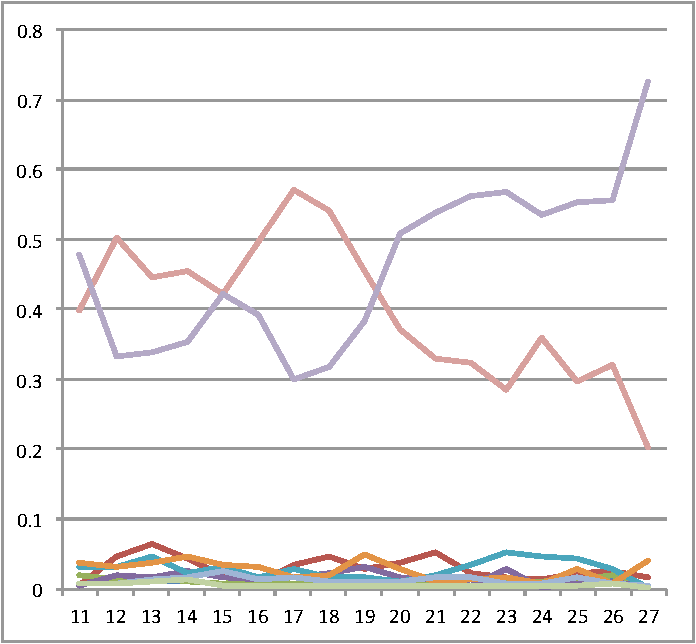
\includegraphics[width=0.48\linewidth]{figures/1LDANews-2.pdf}
\label{fig:news_topics_lda}
}
\subfigure[\stlda]
{
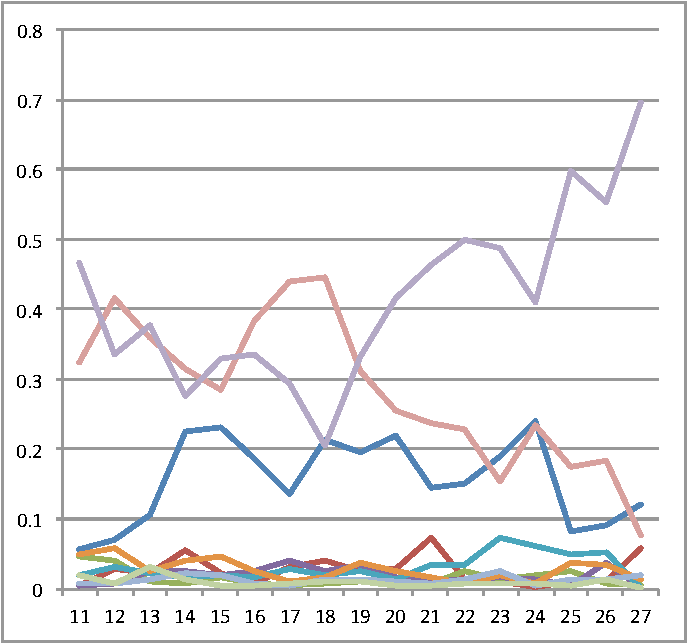
\includegraphics[width=0.48\linewidth]{figures/1STLDANews-2.pdf}
\label{fig:news_topics_stlda}
}
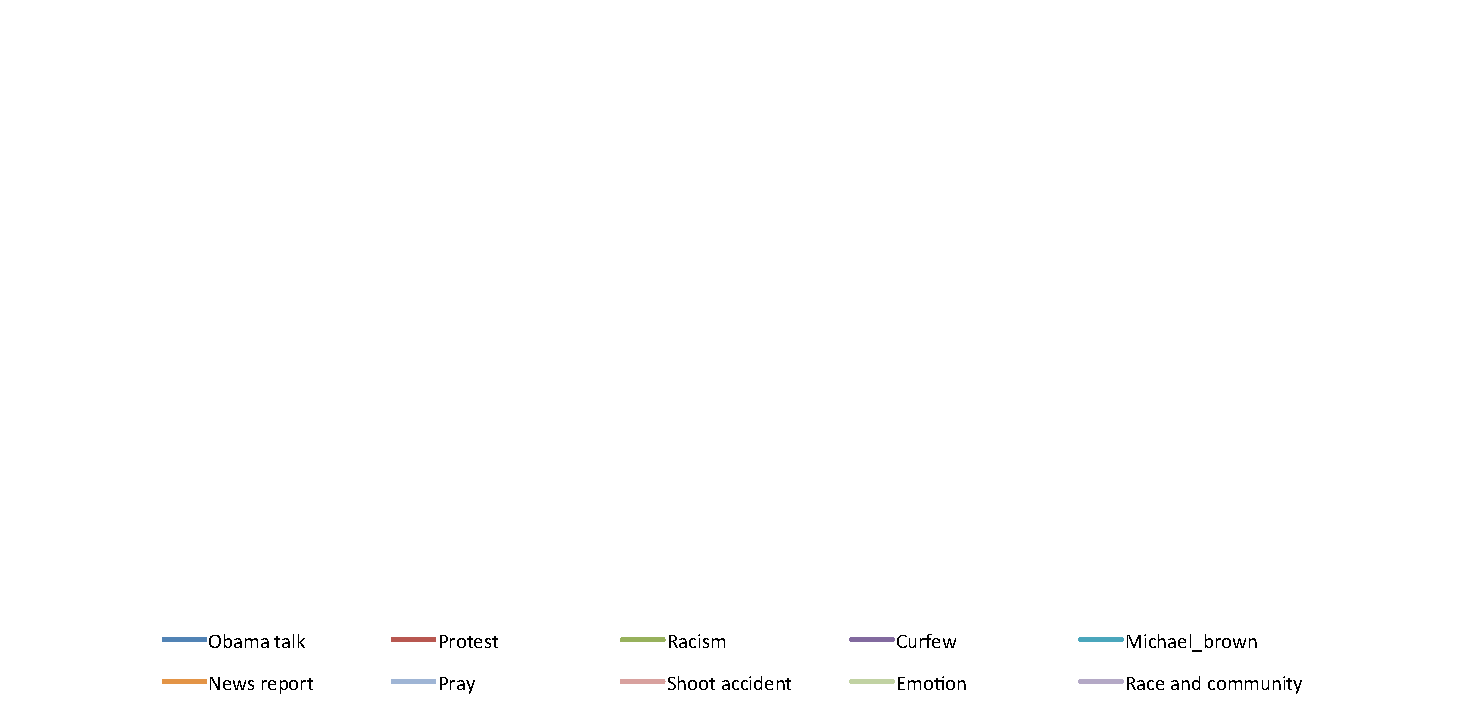
\includegraphics[width=\linewidth]{figures/Legend.pdf}
\caption{News Topic Dynamics by LDA and \stlda}\label{fig:news_topics}
\end{figure*}

Topic distribution given by LDA is highly skewed to two main topics, thus the \emph{Shoot Accident} and the \emph{Race and Community}, while other topics take only a small proportion and it is hard to identify the proportion change of these topics. Meanwhile \stlda gives results that are slightly better in representing different topics. Besides the significant change of \emph{Shoot Accident} and \emph{Race and Community}, the \emph{Obama Talk} is discovered as a main topic for media. It keeps a relatively stable proportion of 20\%, and peaks after some important events related with Obama. For example, on August 12, Obama addressed the shooting and urged the community in Ferguson to stay calm. On August 14, he gave a talk saying there is no excuse for protesters to turn to violence, which seems to lead to the peak on August 14 and 15. Also in news topic dynamics by \stlda, the \emph{Protest} shows a peak on August 21, which is consistent with the date when the National Guard withdrew from the Ferguson.

Both LDA and \stlda are unsupervised methods, so it is hard to verify which topic dynamic reflects the real situation. But the topics discovered by \stlda are more diverse, and are consistent with the important events in the timeline.

There is more variance in topic dynamics of tweets by \stlda than LDA, which is shown in Figure~\ref{fig:tweets_topics}. The proportion of topics is close to each other in topic dynamics by LDA, so it is relatively hard to identify the main topics for each day. There is rising point of \emph{Michael Brown} after the shoot accident, and a peak on August 25 when the funeral for Michael Brown is held. However, consistent with the shortage discussed in analysis of tweet topics, LDA gives a probability distribution of topics, of which some are irrelevant. So when aggregating tweets in a day together, the proportion number for each topic is similar, which makes it hard to identify main topics on that day, and change of topics along the time. Comparatively, \stlda gives results with better representation of topic dynamics. There is variation of topics changing overtime. It is clearly that after the shoot accident, emotion of the public surges to a peak on August 11. After the protest event, another emotion topic appears on August 14. Meanwhile, the proportion of \emph{Pray} topic keeps relatively stable from August 11 to August 24, and increases a lot on the day when Michael Brown's funeral is held. These tendencies in topic changes can be seen in topic dynamics of tweets by LDA, but these topics are entangled with other topics, making it hard to differentiate from other topics.

\begin{figure*}[htpb]
\centering
\subfigure[LDA]
{
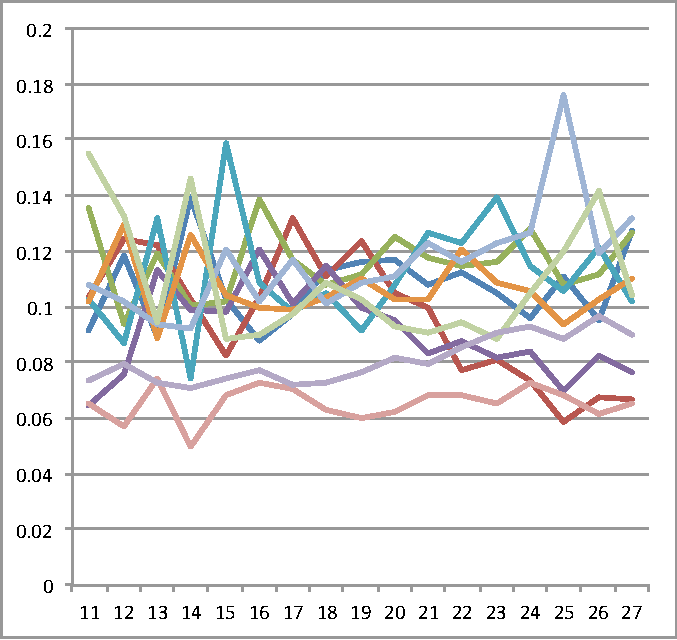
\includegraphics[width=0.48\linewidth]{figures/2LDATweets.pdf}
\label{fig:tweets_topics_lda}
}
\subfigure[\stlda]
{
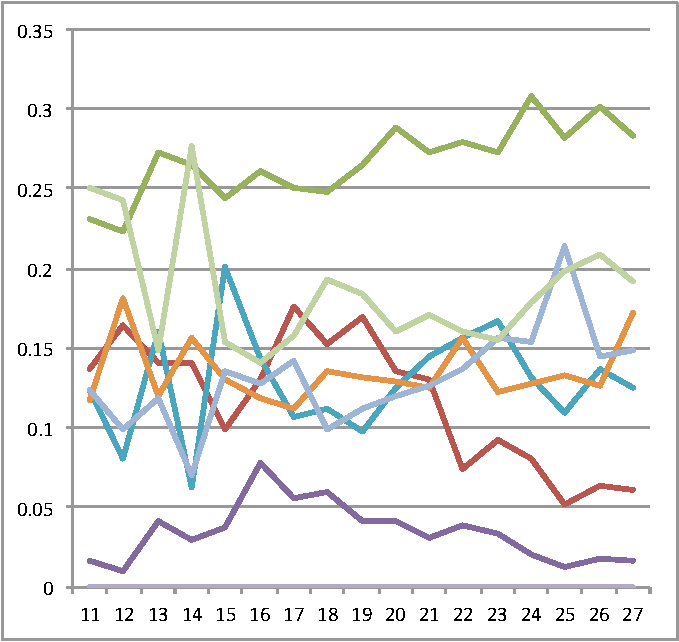
\includegraphics[width=0.48\linewidth]{figures/2STLDATweets.pdf}
\label{fig:tweets_topics_stlda}
}
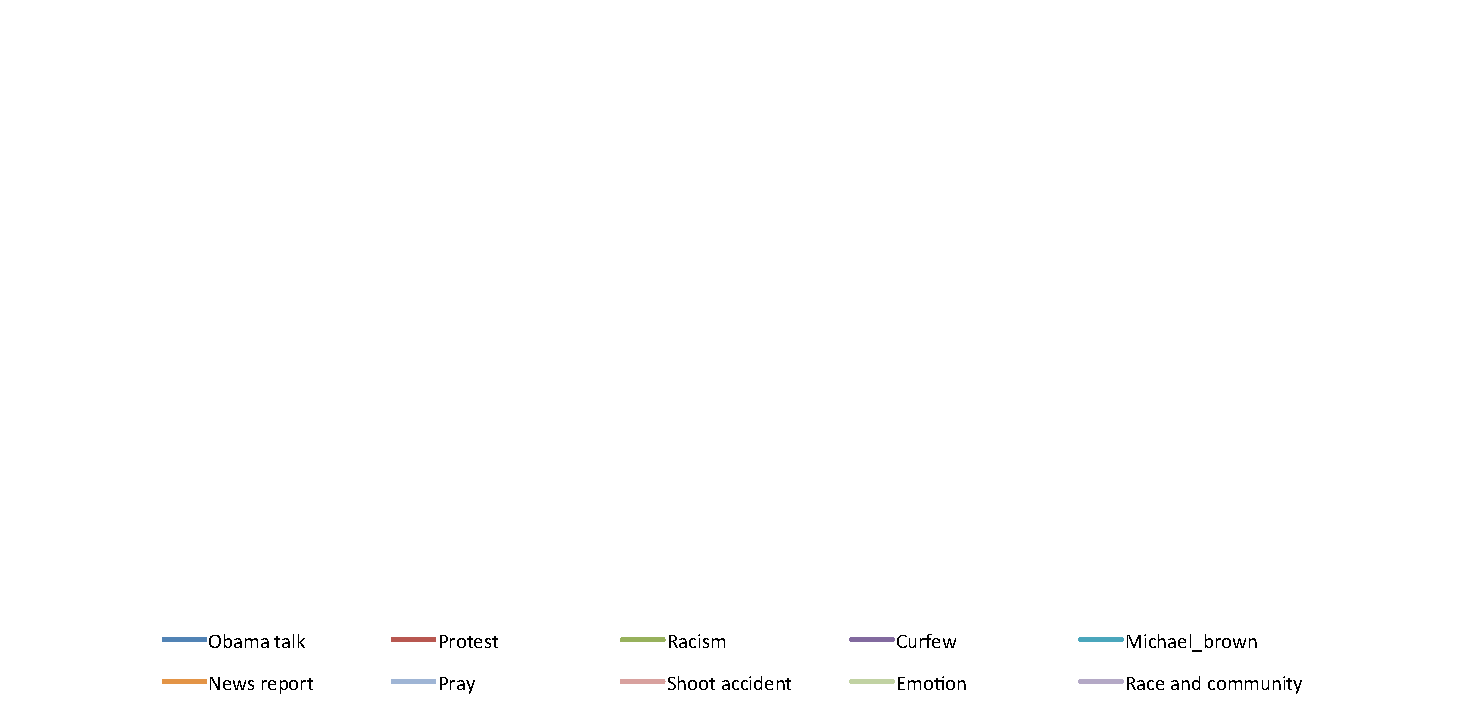
\includegraphics[width=\linewidth]{figures/Legend.pdf}
\caption{Tweets Topic Dynamics by LDA and \stlda}\label{fig:tweets_topics}
\end{figure*}

In summary, by intrinsic and extrinsic evaluation, \stlda is more accurate in assigning one topic to each tweet and giving better results in topic dynamics. %In Section~\ref{subsec:topic_track}, we use the results of \stlda on tweets and news for topic tracking analysis.

\subsection{Topic Tracking}
\label{subsec:topic_track}

In this section, we mainly examine the interaction between news topics and tweets topics by comparing topic dynamics. The interaction between news and tweets is complicated, especially considering the geographic difference in reaction to events.~\newcite{he2015uncovering} find that users in different geographic areas tend to focus differently on an event. In our study, we separate tweets according to geographic boundary of \stlouis where the Ferguson unrest took place. It is assumed that people participating, witnessing or living in nearby areas may behave differently, as reporters, participants or victims. Meanwhile users out of Ferguson area are far away from the place where the event took place, so their knowledge about the event mainly comes from news, social media and other indirect report of the event. The perception of event can be different from people who are experiencing the event. Firstly, we compare topic dynamics in and out of Ferguson area, identifying what the differences are. Secondly, we compare topics in news and tweets. Specifically, we focus on the overlapping topics in news and tweets, examining the topic dynamics and how news or social media opinions may affect each other.

\subsubsection{Tweet Topic Dynamics in and out of \stlouis Area}

The topic dynamics of tweets in and out of \stlouis are shown in Figure~\ref{fig:tweets_topics_stlouis}. Under the common topic frame with news, both tweets in \stlouis area and out of \stlouis area lack some topics that only exist in news, thus topic 0 \emph{Obama Talk}, topic 7 \emph{Shoot Accident} and topic 9 \emph{Race and Community}. For the rest topics, it is obvious that topic change is different for tweets in \stlouis area and out of \stlouis.

\begin{figure*}[htpb]
\centering
\subfigure[In \stlouis]
{
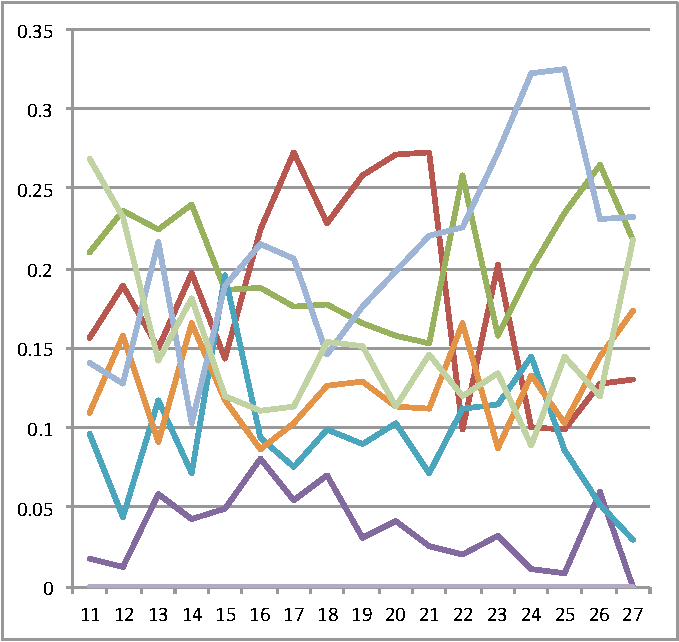
\includegraphics[width=0.48\linewidth]{figures/3LDA2TweetsInSt.pdf}
\label{fig:tweets_topics_inst}
}
\subfigure[Out of \stlouis]
{
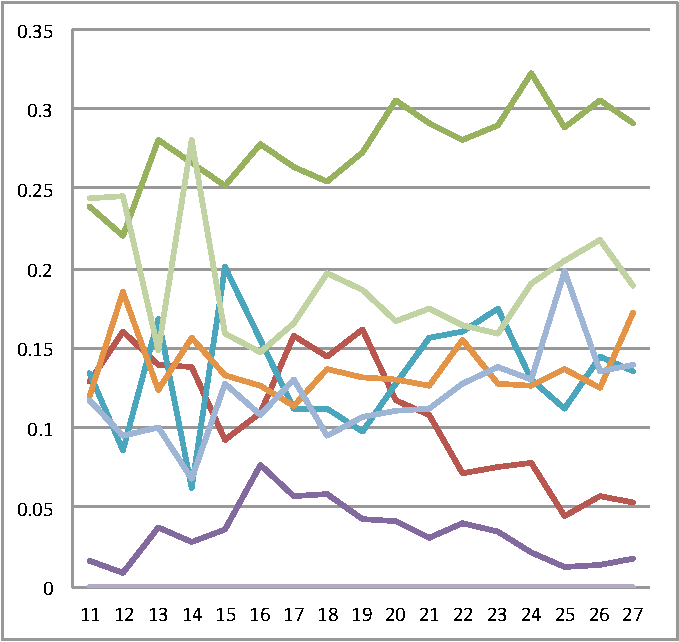
\includegraphics[width=0.48\linewidth]{figures/3LDA2TweetsOutSt.pdf}
\label{fig:tweets_topics_outst}
}
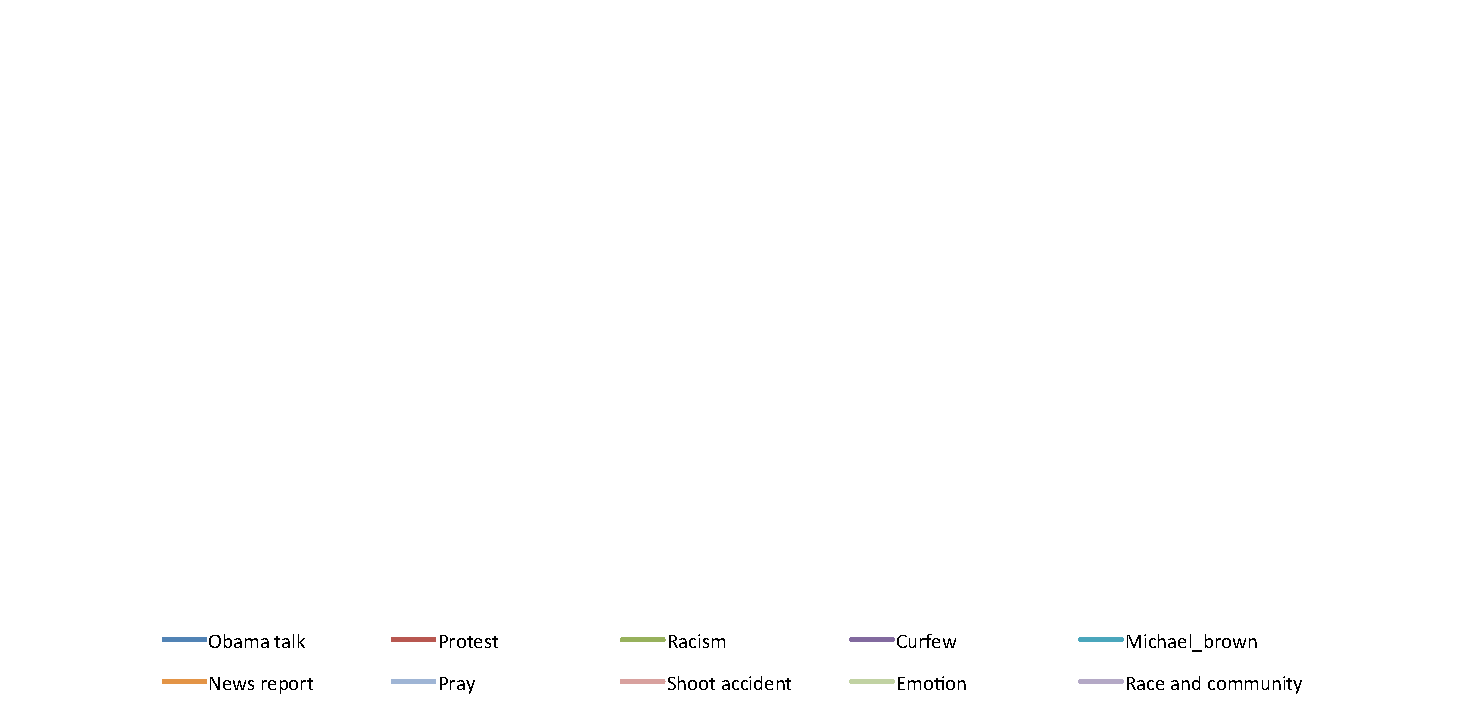
\includegraphics[width=\linewidth]{figures/Legend.pdf}
\caption{Tweets Topic Dynamics in and out of \stlouis by \stlda}\label{fig:tweets_topics_stlouis}
\end{figure*}

The proportion of tweets talking about \emph{Curfew} increases to 7.5\%, which is a peak on August 18 and then decreases. This topic change is similar for both tweets in and out of \stlouis area. Meanwhile the proportion of tweets talking about \emph{News Report} and \emph{Michael Brown} are similar along the time. Tweets about \emph{News Report} keep taking about 10\% to 15\% of all tweets. There are three small peaks on August 12, 14 and 22. Proportion of tweets talking about \emph{Michael Brown} and emph{Shoot Accident} increases a lot on August 15 in and out Ferguson area. It may be caused by the release of video recording Brown in a robbery prior to being shot. The public, both in and out of Ferguson area can be affected by it and begin to discuss a lot about it.

Difference lies in topic proportion of \emph{Pray}, but they share similar dynamics. Both in and out of \stlouis area, the increase of tweets with \emph{Pray} topic is consistent with the time when Michael Brown's funeral is held. On August 25, more than 35\% of tweets in Ferguson are about \emph{Pray}. Out of \stlouis, the number of tweets about \emph{Pray} increases to a peak on that day, taking 20\% of all.

It is reasonable to find that more tweets in \stlouis talk about \emph{Protest}, while out of \stlouis more tweets talk about \emph{Racism}. From August 18, when Governor Nixon deployed the National Guard to Ferguson, to August 21 when the National Guard withdrew, protests and conflicts keep occurring. People in Ferguson area are closer and more related to protests, so tweets with this topic surge to take more than 25\% of all tweets. Meanwhile proportion of \emph{Protest} tweets out of \stlouis is far less. The public who are not involved in the event tend to have less knowledge about real situations, but according to what they hear and know, they are better at abstract thinking about this event, thus \emph{Racism} takes majority in most of the time.

An interesting phenomenon is the \emph{Emotion} topic change. Michael Brown was killed on August 9, and anger emotion is the major topic of tweets in \stlouis, then \emph{Emotion} tweets keep decreasing, taking 10\% to 15\% of all tweets. However outside \stlouis area, there is a lag effect of \emph{Emotion} explosion. It is possible that news takes time to spread and the public outside Ferguson need more information to understand what happened. Besides, outsiders may care more about the conflicts between protesters and police, so their emotion was detonated when protests began.

Comparison of topic dynamics in and out of \stlouis area shows that, the public in \stlouis tends to publish tweets that are more related with evlovement of event, such as the shooting, protests and funeral. Meanwhile people out of \stlouis area has lag effect in \emph{Emotion} explosion and have more abstract perception on events, thus \emph{Racism} tweets take a majority. They share similar amount of focus on \emph{News Reports}, investigation of \emph{Michael Brown Shooting Accident} and \emph{Curfew}, which might because these issues are not quite closely related to them, or the influence is relatively small.

\subsubsection{Topic Dynamics of News and Tweets}

Using the results of \stlda, we compare the topics of news and tweets both in and out of \stlouis area. We observe that the three main topics in news, \emph{Obama Talk}, \emph{Shoot Accident} and \emph{Race and Community}, do not exist in tweets. However corresponding to shoot accident investigation, there is similar topic \emph{Michael Brown}, which is a main topic in tweets, taking a small proportion in news. Although the thing news and tweets talk about is the same, how they talk and what words they use is quite different, so it is identified with two separate topics for news and tweets. Similarly, \emph{Racism} topic exists mostly in tweets, while \emph{Race and Community} mainly exists in news. Although these two topics are talking about race, there is little overlapping of tweets and news in the two topics. It indicates that media and the public are using quite different words to discuss the same thing. One possible reason is that tweets use more oral language, while news uses more formal written language. It is also possible that media and the public describe the same thing with different frames. According to the top words in two topics, there are more negative words in \emph{Racism} such as \emph{stop}, \emph{riot}. In the topic labeled with \emph{Race and Community}, words like \emph{make}, \emph{good}, \emph{community} are indicative of positive emotion. Thus the public tends to have negative emotion about race issues during the Ferguson unrest, but the media tried to describe and lead the discussion to a positive way.

Two topics in tweets have little proportion in news, which are \emph{Emotion} and \emph{Prays}. It is reasonable that tweets are more subjective and contain more words about feelings, emotions and prays, while news is more serious and should be objective, avoiding emotional leadings. So the topic difference in tweets and news reflects the characteristics of two types of documents.

Another difference in news and tweets is topic diversity. Comparing topic dynamics of news (Figure~\ref{fig:news_topics_stlda}) and that of tweets (Figure~\ref{fig:tweets_topics_stlda}), it is obvious that tweets have more diverse topics, and proportion of different topics changes overtime. But there are only three main themes in news, and the changing of topics is rare. Topic related with Obama keeps a stable proportion in news report, while the report of investigation, and discussion of race issues keeps alternating dominance. The results show that public topics change along with evolvement of events, while media has certain issues to cover. Public opinions are more diverse. Under certain issues, voice of certain topic could become mainstream.

The overlapping topics between news and tweets are \emph{Protest}, \emph{Curfew}, \emph{Michael Brown} and \emph{News Report}, which are shown in Figure~\ref{fig:topics_news_tweets}. We compare dynamics of these topics for news and tweets separately in and out of \stlouis area. For better observation of trend, we use smoothed line here instead of linear connection between points. The topic dynamic shapes for \emph{Protest} of news and tweets seem to be similar. \emph{Protest} has peaks on almost the same day for three sets of document, while \emph{Curfew} peak in news seems to have a slight lag after tweets. It is possible that people in Ferguson are under curfew and reporting it timely, but news may take some time to process information and publish.

\begin{figure*}[htpb]
\centering
\subfigure[Protest]
{
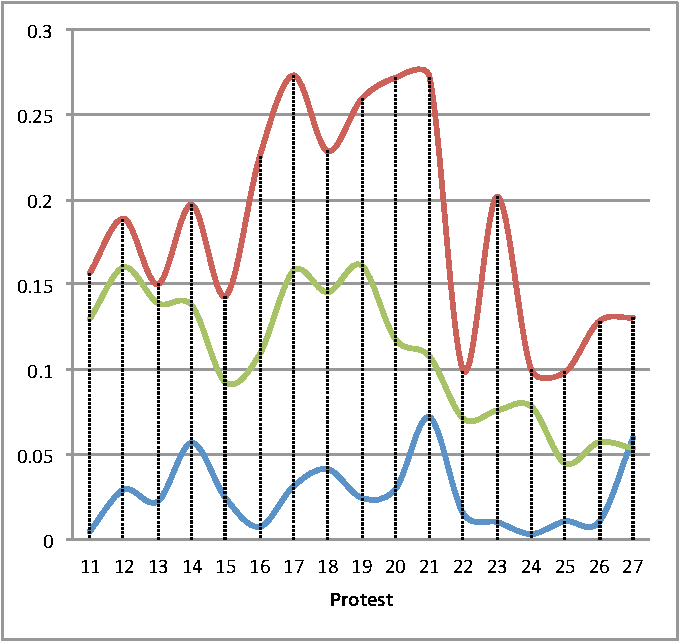
\includegraphics[width=0.48\linewidth]{figures/4_1_Protest.pdf}
\label{fig:protest}
}
\subfigure[Curfew]
{
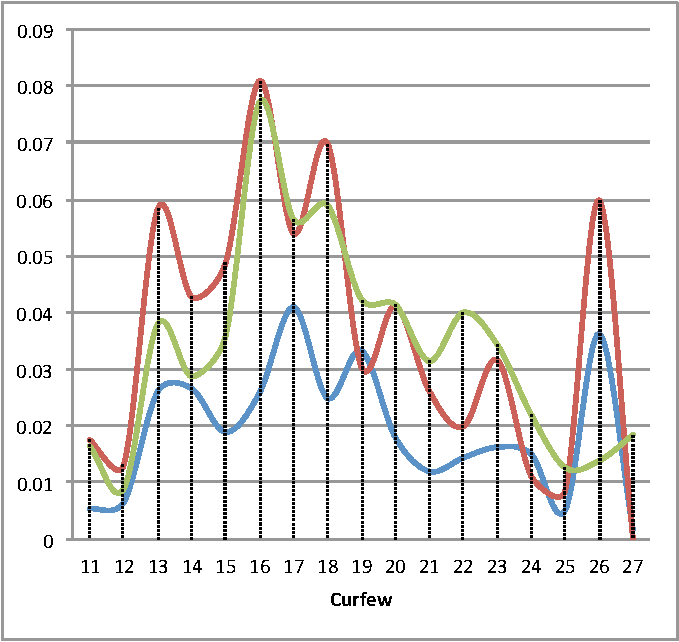
\includegraphics[width=0.48\linewidth]{figures/4_2_Curfew.pdf}
\label{fig:curfew}
}
\subfigure[Michael Brown]
{
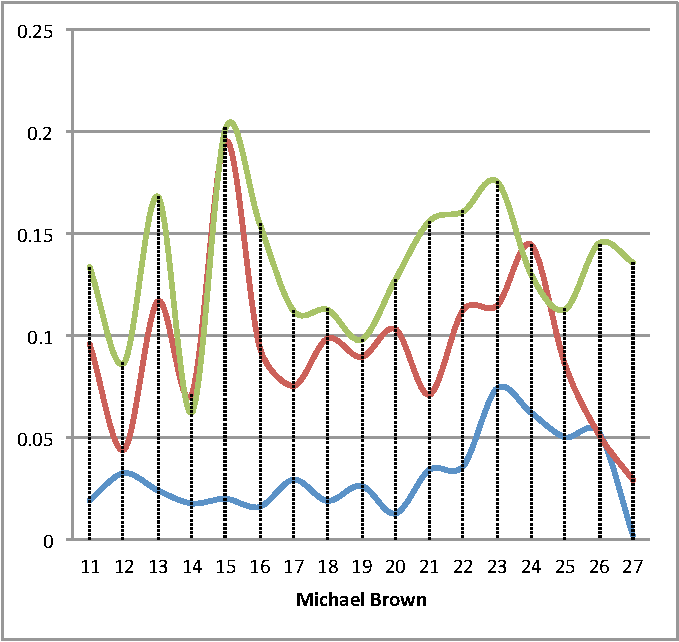
\includegraphics[width=0.48\linewidth]{figures/4_3_Michael_Brown.pdf}
\label{fig:mb}
}
\subfigure[News Report]
{
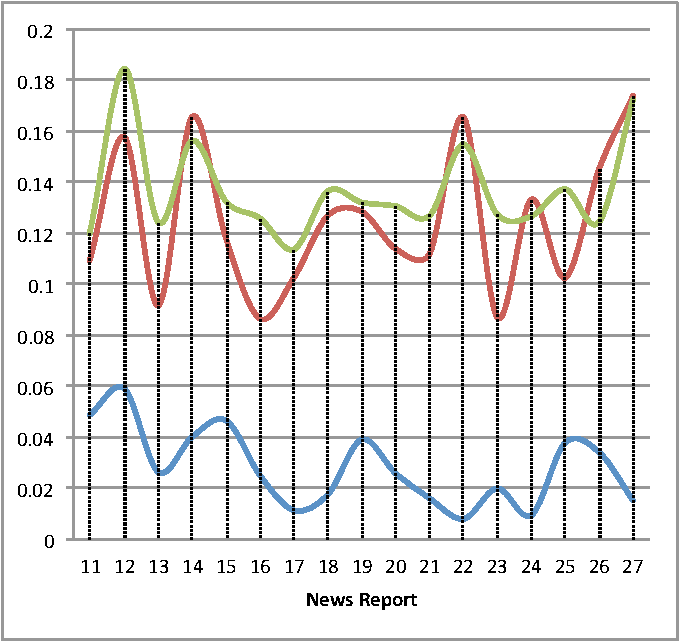
\includegraphics[width=0.48\linewidth]{figures/4_4_News_report.pdf}
\label{fig:news_report}
}
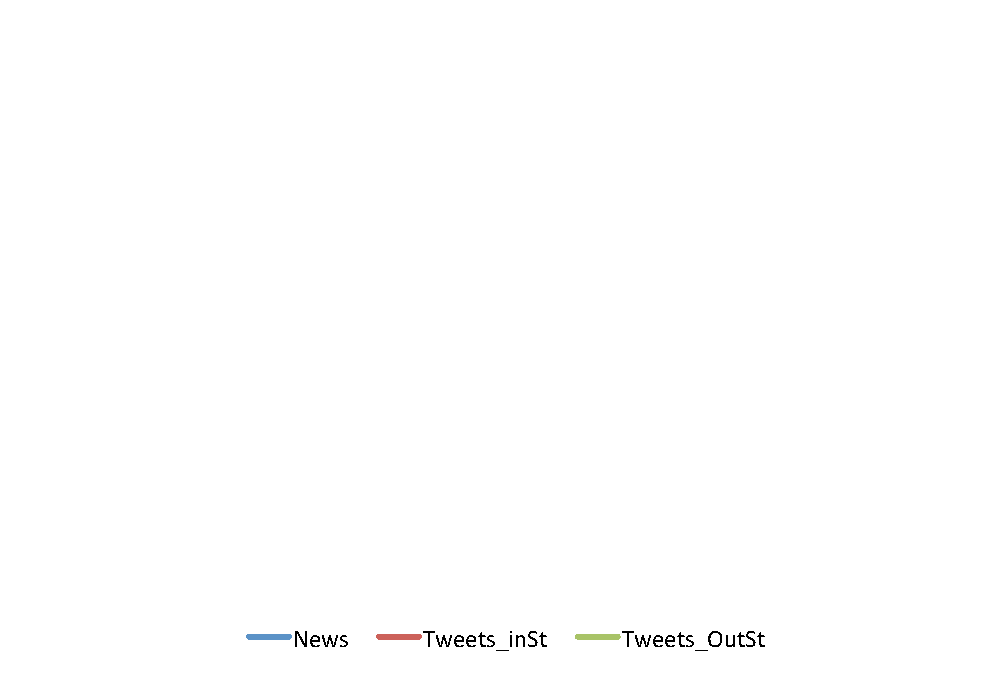
\includegraphics[width=0.5\linewidth]{figures/4_Legend_cut.pdf}
\caption{Topic Dynamic of News and Tweets by \stlda}\label{fig:topics_news_tweets}
\end{figure*}

There is no common pattern in \emph{Michael Brown}. According to analysis above, news mainly focus on investigation and getting to the bottom of shoot accident, which is labeled \emph{Shoot Accident}. It is talking about the same thing as topic \emph{Michael Brown}, however the words they use are quite different. So \emph{Michael Brown} topic has a tiny proportion in news, which takes less than 5\%.

For the topic \emph{News Report}, there is time difference in peaks of topic for news and tweets. However it is hard to know whether tweets cite some report first, and media is influenced to cite report, or in the other way around, or there may be no relation at all.

